\documentclass[conference]{IEEEtran}
\IEEEoverridecommandlockouts
% The preceding line is only needed to identify funding in the first footnote. If that is unneeded, please comment it out.
\usepackage{cite}
\usepackage{amsmath,amssymb,amsfonts}
\usepackage{graphicx}
\usepackage{textcomp}
\usepackage{xcolor}
\usepackage{titlesec}

\usepackage{textcomp}
\usepackage{epsfig}
\usepackage{algpseudocode}
\usepackage{pgfplots}
\usepackage{tikz}
\pgfplotsset{width=10cm,compat=1.9}
 \usepgfplotslibrary{external}
\usepackage{amsmath}
\usepackage{mathtools}
\DeclarePairedDelimiter{\floor}{\lfloor}{\rfloor}
\usepackage[linesnumbered,ruled,vlined]{algorithm2e}
\def\BibTeX{{\rm B\kern-.05em{\sc i\kern-.025em b}\kern-.08em
    T\kern-.1667em\lower.7ex\hbox{E}\kern-.125emX}}

\usepackage[ruled,vlined]{algorithm2e}

\tikzexternalize 
\begin{document}

\title{An Algorithm to find the element present at k'th position  in two sorted arrays.\\
\text{\Large{DAA ASSIGNMENT-1 , GROUP 2}}
}
\author{\IEEEauthorblockN{Vasu Gupta}
\IEEEauthorblockA{ \text{IIB2019003}}
\and
\IEEEauthorblockN{Saloni Singla}
\IEEEauthorblockA{ \text{IIB2019004}}
\and
\IEEEauthorblockN{Sandeep Kumar}
\IEEEauthorblockA{ \text{IIB2019005}}
}

\maketitle

\begin{abstract}
This Paper contains the algorithm for finding the element that would be at the k'th position of the final sorted array generated from given two arrays of size m and n.
\end{abstract}

\section{Problem Statement}
Given two sorted arrays of size m and n respectively, you are tasked
with finding the element that would be at the k’th position of the
final sorted array.

\section{Keywords}
Arrays, Sorting, Divide and Conquer

\section{Introduction}
Let’s  first  formally  define  what Divide and conquer algorithm is.\\
The Divide and conquer strategy solves a problem by:
\begin{enumerate}
\item Divide: Breaking the problem into sub problems that are themselves smaller instances of the same type of problem.
\item Recursion: Recursively solving these sub-problems.
\item Conquer: Appropriately combining their answers.
\end{enumerate}
\section{Algorithmic Design}

\subsection{ \textbf{Approach 1}}
\begin{enumerate}
\item  If  the value of k is greater than sum of n and m or k is less than 1 then return -1. 
\item  If one of the array is empty then return the element present at $\displaystyle{\left({k}-{1}\right)}^{{{t}{h}}}$ position in the other array.
\item If value of k is equal to 1 then return the minimum among the arr1[0] and arr2[0].
\item Store the minimum among n and k/2  \& m and k/2 in i and j respectively (we are comparing size of arrays with k/2 to avoid Segmentation Fault if k/2 is greater than size of array).
\item In this divide and conquer approach we will divide both the arrays arr1[] and arr2[] by half of the value of k and then recurse the function.
\end{enumerate}

\subsection{ \textbf{Approach 2}}
\begin{enumerate}
\item  If  arr1 is equal to end1 then return the element present at $\displaystyle{\left({k}\right)}^{{{t}{h}}}$ in arr2[].
\item If  arr2 is equal to end1 then return the element present at $\displaystyle{\left({k}\right)}^{{{t}{h}}}$  in arr1[].
\item Calculate the mid-points of the arr1[] and arr2[]. 
\item Lets make an assumption that element present at mid-point of arr1 is less than k then it is clear that the elements after mid-point of arr2[] cannot be the  $\displaystyle{\left({k}\right)}^{{{t}{h}}}$ element.
\item So according to our assumption we will set the element present at mid-point of arr2[] as the last element of the arr2[].
\item In this way,we will get a new sub-problem with half the size of one of the arrays.
\end{enumerate}

\newline
\begin{algorithm}
    \caption{To find the $\displaystyle{k}'{t}{h}$ element in the final sorted array}
    \KwIn{ Two arrays arr1 and arr2 of size n and m respectively and k such that $\displaystyle{0}<{k}<{m}+{n}+{1}$}
    \KwOut {Return the element at the $\displaystyle{k}'{t}{h}$ position}
    \DontPrintSemicolon
    \SetKwFunction{FMain}{Kth}
    \SetKwProg{Fn}{Function}{:}{}
    \Fn{\FMain{$arr1$,$arr2$,$m$,$n$,$k$}}{
        
        \If{ k \textgreater{} m+n or k $\displaystyle<$ 1}{
            \STATE\Return{$-1$}
        }
        \If{ m = 0  and n \textgreater{} 0}{
        	   \STATE\Return{$arr2[k-m-1]$}
               }
        \If{ n = 0  and m \textgreater{} 0}{
        		\STATE\Return{arr1[k-n-1]}
               }
        \If{ k = 1}{
             	\STATE\Return{minimum(arr1[0],arr2[0])}
               }
          \STATE $i\gets minimum(m,k/2)$
          \STATE $j\gets minimum(n,k/2)$
          
         \eIf{$\displaystyle{a}{r}{r}{1}{\left[{i}-{1}\right]}<{a}{r}{r}{2}{\left[{j}-{1}\right]}$}{
   				\STATE\Return{\Call{$\displaystyle{k}{t}{h}$}{$ arr1 + i $,$ arr2 $, $m - i$ , $ n,k - i $}}\;
  			 }{
   				\STATE\Return{\Call{$\displaystyle{k}{t}{h}$}{$arr1$,$ar2 + j $,$ m $, $n - j$, $k - j$}}
  			 }      
    }
\end{algorithm}

\begin{algorithm}
    \caption{To find the $\displaystyle{k}'{t}{h}$ element in the final sorted array}
    \KwIn{ Two arrays arr1 and arr2 of size n and m respectively and k such that $\displaystyle{0}<{k}<{m}+{n}+{1}$}
    \KwOut {Return the element at the $\displaystyle{k}'{t}{h}$ position}
    \DontPrintSemicolon
    \SetKwFunction{FMain}{Kth}
    \SetKwProg{Fn}{Function}{:}{}
    \Fn{\FMain{$array1$,$array2$,$end1,$end2,$k-1$}}{
        \If{ array1 = end1 }{
        	   \STATE\Return{$array2[k]$}
               }
        \If{ array2 = end2 }{
        		\STATE\Return{array1[k]}
               }
          \STATE $mid1\gets (end1-array1)/2$
          \STATE $mid2\gets (end2-array2)/2$\\
          \eIf{mid1+mid2 $\displaystyle<$ k}{
                \eIf{array1[mid1 $\displaystyle>$ array2[mid2]}{
                   \STATE\Return{\Call{$\displaystyle{k}{t}{h}$}{$array1$,$array2+mid2+1$, $end1$,$end2$,$k-mid2-1$}}
                   }{
                   \STATE\Return{\Call{$\displaystyle{k}{t}{h}$}{$array1+mid1+1$,$array2$, $end1$,$end2+mid2$,$k-mid1-1$}}
                  }
               }{
               \eIf{array1[mid1] $\displaystyle>$ array2[mid2]}{
                   \STATE\Return{\Call{$\displaystyle{k}{t}{h}$}{$array1$,$array2$, $array1+mid1$,$end2$,$k$}}
                   }{
                   \STATE\Return{\Call{$\displaystyle{k}{t}{h}$}{$array1$,$array2$, $end1$,$array2+mid2$,$k$}}
                  }
               }
               
    }     
   
\end{algorithm}
\newpage
% Continue.....

\section{Algorithm Analysis}

\subsection{\textbf{Approach 1}} 
\textbf{Time Complexity Analysis}
\\In this recursive divide and conquer approach, the function kth is called a total of logm+logn  times. Thus the time complexity of this approach would be $\displaystyle{O}{\left( \log{{k}}\right)}$. The best case complexity will be when either of m and n is zero or k is invalid or k is equal to 1. Thus, the best case time
complexity is  \displaystyle\[\Omega\](1)
\newline
\textbf{Space Complexity Analysis}
\\This algorithm has a space complexity of O(log k)

\subsection{\textbf{Approach 2}} 
\textbf{Time Complexity Analysis}
\\In this recursive divide and conquer approach, the function kth is called log k times. Thus the time complexity of this approach would be $\displaystyle{O}{\left( \log{{m}}+ \log{{n}}\right)}$ . \newline The best case complexity will be when either of m and n is zero or k is invalid or k is equal to 1. Thus, the best case time
complexity is  \displaystyle\[\Omega\](1)
\newline
\textbf{Space Complexity Analysis}
\\This algorithm has a space complexity of O(log m+log n)

\section{Experimental study}

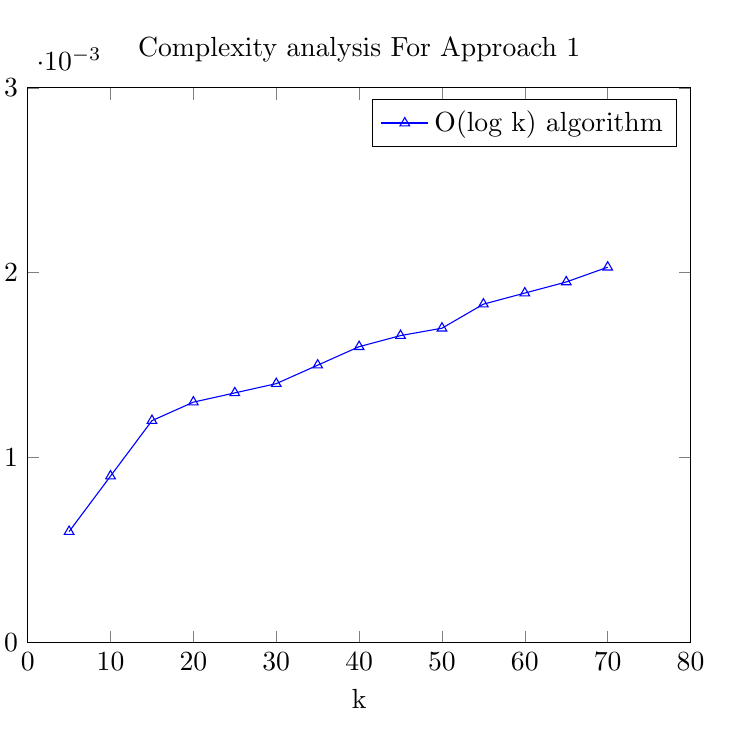
\begin{tikzpicture}[trim left=0cm]
\begin{axis}[
    title={Complexity analysis For Approach 1 },
    xlabel={k},
    ylabel={Time taken in (ms)},
    xmin=0, xmax=80,
    ymin=0, ymax=0.0030,
    xtick={0,10,20,30,40,50,60,70,80},
    ytick={0,0.0010, 0.0020, 0.0030,0.0040,0.0050}
]

\addplot[
    color=blue,
    mark=triangle,
    ]
    coordinates {
    (5,0.0006)(10,0.0009)(15,0.0012)(20,0.0013)(25,0.00135)(30,0.0014)(35,0.0015)(40,0.0016)(45,0.00166)(50,0.0017)(55,0.00183)(60,0.00189)(65,0.00195)(70,0.00203)
    
    };
    \legend{O(log k) algorithm}
   \end{axis}
   
\end{tikzpicture}



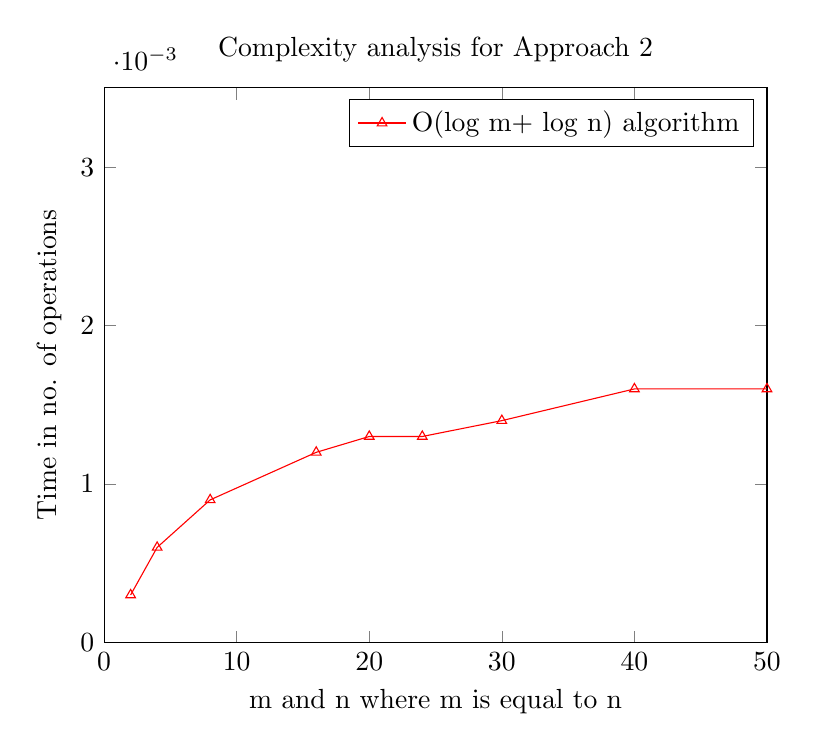
\begin{tikzpicture}
\begin{axis}[
    title={Complexity analysis for Approach 2},
    xlabel={m and n where m is equal to n},
    ylabel={Time in no. of operations},
    xmin=0, xmax=50,
    ymin=0, ymax=0.0035,
    xtick={0,10,20,30,40,50},
    ytick={0,0.0010, 0.0020, 0.0030},
]

\addplot[
    color=red,
    mark=triangle,
    ]
    coordinates {
    (2, 0.0003)(4,0.0006)(8,0.0009)(16,0.0012)(20,0.0013)(24,0.0013)(30,0.0014)(40,0.0016)(50,0.0016)
    };
    \legend{O(log m+ log n) algorithm}
  \end{axis}
  \end{tikzpicture}
  
\section{Conclusion}
Above two methods have different time complexities and meet to fulfill the problem statement. The order in which they are good can be listed as:
\\I. Approach 1
\\II. Approach 2
\\Based on the time complexities.
\section{REFERENCES}
\textit{https://www.geeksforgeeks.org/k-th-element-two-sorted-arrays/}\\
\textit{https://tutorialspoint.dev/algorithm/divide-and-conquer/k-th-element-two-sorted-arrays}\\

\end{document}
